% ==================================================================================
% W-STTran Method — Detailed Technical Report
% Target Venue: NeurIPS
% ==================================================================================
\documentclass{article}

% Uncomment if neurips_2026.sty is available
% \usepackage[preprint]{neurips_2026}
% Fallback to standard margins if neurips is unavailable:
\usepackage[margin=1in]{geometry}

\usepackage[utf8]{inputenc}
\usepackage{amsmath,amssymb,amsfonts}
\usepackage{graphicx}
\usepackage{booktabs}
\usepackage{algorithm}
\usepackage{algpseudocode}
\usepackage{bm}
\usepackage{xcolor}
\usepackage{tikz}
\usetikzlibrary{arrows.meta,positioning,shapes.geometric,fit,calc,backgrounds}

\newcommand{\mR}{\mathbb{R}}
\newcommand{\op}[1]{\operatorname{#1}}
\newcommand{\mat}[1]{\bm{#1}}

\title{W-STTran: A Minimal Baseline for World Scene Graph Generation}
\author{Anonymous Authors}

\begin{document}

\maketitle

% ====================================================================================
\section{Introduction}
\label{sec:intro}
% ====================================================================================

The W-STTran architecture provides a minimal baseline adaptation of the STTran video scene graph generation method to the World Scene Graph Generation (WorldSGG) task. Standard video scene graph methods operate purely in 2D image space and reason only about objects currently visible in the camera frame. W-STTran extends this paradigm by anchoring predictions in a persistent 3D world coordinate frame using an explicit memory buffer.

W-STTran serves to test whether passive memory combined with 3D spatial attention is sufficient to solve the WorldSGG task. It utilizes a FasterRCNN-ResNet50 backbone for monocular 3D detection and visual feature extraction. Crucially, it does \emph{not} include explicit object tracking mechanisms, camera or motion encoders, or temporal edge attention, making it the most stripped-down baseline in our comparative study.

% ====================================================================================
\section{Pipeline Overview}
\label{sec:pipeline}
% ====================================================================================

The complete dataflow for W-STTran is illustrated in Figure~\ref{fig:pipeline_wsttran}. Features from the monocular 3D detector are buffered, enriched with 3D geometric scaffolding, tokenized, and passed through a global spatial transformer to produce the final relationship predictions.

\begin{figure}[h]
\centering
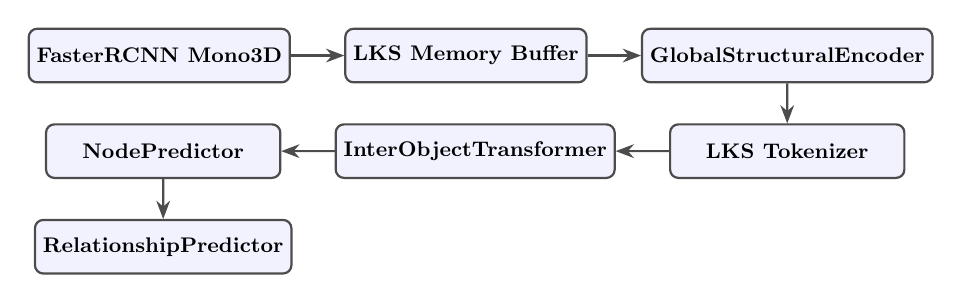
\begin{tikzpicture}[
  scale=0.85, transform shape, >=Stealth,
  block/.style={draw=black!70, rounded corners=3pt, line width=0.8pt, fill=blue!5, minimum width=3.5cm, minimum height=0.8cm, font=\small\bfseries, align=center},
  arrow/.style={->, thick, black!70}
]

\node[block] (mono) {FasterRCNN Mono3D};
\node[block, right=0.8cm of mono] (buffer) {LKS Memory Buffer};
\node[block, right=0.8cm of buffer] (gse) {GlobalStructuralEncoder};
\node[block, below=0.6cm of gse] (tok) {LKS Tokenizer};
\node[block, left=0.8cm of tok] (iot) {InterObjectTransformer};
\node[block, left=0.8cm of iot] (np) {NodePredictor};
\node[block, below=0.6cm of np] (rp) {RelationshipPredictor};

\draw[arrow] (mono) -- (buffer);
\draw[arrow] (buffer) -- (gse);
\draw[arrow] (gse) -- (tok);
\draw[arrow] (tok) -- (iot);
\draw[arrow] (iot) -- (np);
\draw[arrow] (np) -- (rp);

\end{tikzpicture}
\caption{The W-STTran pipeline. Visual features and 3D geometries are buffered and combined via the Tokenizer, followed by global inter-object reasoning and relationship prediction.}
\label{fig:pipeline_wsttran}
\end{figure}


% ====================================================================================
\section{LKS Memory Buffer}
\label{sec:lks}
% ====================================================================================

The LKS (Last Known State) Memory Buffer is a non-differentiable zero-order hold that provides object persistence. It operates on raw visual features $\mat{f}_n^{(t)}$ extracted by the FasterRCNN backbone. For each object $n$ at frame $t$:
\begin{equation}
    \mat{m}_n^{(t)} = \begin{cases}
        \mat{f}_n^{(t)} & \text{if object $n$ is visible at $t$}, \\
        \mat{f}_n^{(\tau^*)} & \text{where } \tau^* = \arg\min_{\tau:\text{vis}(n,\tau)} |t - \tau|, \\
        \bm{0} & \text{if object $n$ is never seen}.
    \end{cases}
    \label{eq:lks_buffer}
\end{equation}
The nearest visible frame $\tau^*$ is found using a bidirectional nearest-neighbor search, implemented efficiently via vectorized forward and backward \texttt{cummax} operations over the temporal axis.

The buffer also outputs a staleness value $\Delta_n^{(t)} = |t - \tau^*|$, representing the temporal distance to the last observation. For objects that are never seen, a sentinel value of $\Delta=1000$ is assigned to decouple the feature from the video length.


% ====================================================================================
\section{GlobalStructuralEncoder}
\label{sec:gse}
% ====================================================================================

To ground the buffered visual features in the 3D world geometry, the \emph{GlobalStructuralEncoder} converts 3D oriented bounding boxes (OBBs) into per-object structural tokens.

An OBB is defined by its 8 corner vertices $\mat{C}_n \in \mR^{8 \times 3}$. We first center each box to obtain a translation-invariant local geometry:
\begin{align}
    \bar{\mat{c}}_n &= \frac{1}{8}\sum_{i=1}^{8}\mat{c}_{n,i} \in \mR^{3}, \label{eq:center} \\
    \tilde{\mat{c}}_{n,i} &= \mat{c}_{n,i} - \bar{\mat{c}}_n \in \mR^{3}, \quad i=1,\dots,8. \label{eq:local}
\end{align}
The local corners are flattened and concatenated with the absolute center to form a 27-dimensional input $\mat{x}_n$. A shared multi-layer perceptron (MLP) processes this geometry to produce a structural token:
\begin{equation}
    \mat{g}_n = \op{MLP}_{\text{obj}}\bigl(\mat{x}_n\bigr) \in \mR^{d_{\text{struct}}}.
    \label{eq:gse_obj}
\end{equation}

A permutation-invariant global scene summary is also computed via max-pooling over the valid objects $\mathcal{V}$:
\begin{equation}
    \mat{g}_{\text{global}} = \op{MLP}_{\text{global}}\!\Bigl(\max_{n \in \mathcal{V}} \mat{g}_n\Bigr) \in \mR^{d_{\text{struct}}}.
    \label{eq:gse_global}
\end{equation}


% ====================================================================================
\section{LKS Tokenizer}
\label{sec:tokenizer}
% ====================================================================================

The Tokenizer fuses the 3D geometry from the structural encoder, the buffered visual features, and the staleness metadata into a unified token:
\begin{equation}
    \mat{x}_n^{(t)} = \op{FusionProj}\bigl([\mat{g}_n^{(t)} \;\|\; \mat{m}_n^{(t)} \;\|\; \log(\Delta_n^{(t)} + 1)]\bigr) \in \mR^{d_{\text{model}}}.
    \label{eq:pwg_tokenizer}
\end{equation}
The fusion is performed by a linear projection followed by LayerNorm and GELU activation. Since W-STTran does not use camera features, they are omitted from the concatenation.


% ====================================================================================
\section{InterObjectTransformer}
\label{sec:iot}
% ====================================================================================

Global intra-frame spatial reasoning is handled by the \emph{InterObjectTransformer}. This module is a vanilla Transformer encoder applied across all valid objects in a frame.

Instead of standard 1D positional encoding, we compute continuous pairwise spatial positional encodings based on 3D distances and volumes:
\begin{align}
    d_{ij} &= \sqrt{\|\bar{\mat{c}}_i - \bar{\mat{c}}_j\|^2 + 10^{-6}}, \label{eq:dist} \\
    \hat{\mat{d}}_{ij} &= \frac{\bar{\mat{c}}_i - \bar{\mat{c}}_j}{d_{ij}} \in \mR^{3}, \label{eq:dir} \\
    \rho_{ij} &= \log V_i - \log V_j, \label{eq:volratio}
\end{align}
where $V_n$ is the exact OBB volume. The 5-dimensional pairwise features are processed by an MLP and mean-aggregated over neighbors to form the additive spatial positional encoding $\mat{S}^{(t)}$:
\begin{equation}
    \mat{s}_i = \op{Linear}\Bigg(\frac{1}{|\mathcal{N}_i|}\sum_{j \in \mathcal{N}_i}\op{MLP}_{\text{pair}}\bigl([d_{ij},\,\hat{\mat{d}}_{ij},\,\rho_{ij}]\bigr)\Bigg) \in \mR^{d_{\text{model}}}.
    \label{eq:spe}
\end{equation}

The tokens are then updated via self-attention:
\begin{equation}
    \mat{H}^{(t)} = \op{TransformerEncoder}\bigl(\mat{X}^{(t)} + \mat{S}^{(t)},\; \text{mask}=\overline{\mat{v}}^{(t)}\bigr) \in \mR^{N \times d_{\text{model}}}.
    \label{eq:iot_attn}
\end{equation}
We use a Pre-LN architecture with a validity-based padding mask $\overline{\mat{v}}^{(t)}$ to ignore non-existent objects.


% ====================================================================================
\section{Node Predictor}
\label{sec:node_pred}
% ====================================================================================

The updated node representations are passed to the Node Predictor, a two-layer MLP with ReLU activation and Dropout, which outputs object classification logits:
\begin{equation}
    \hat{\mat{y}}_n^{\text{obj}} = \op{MLP}_{\text{node}}(\mat{h}_n) \in \mR^{C_{\text{obj}}},
    \label{eq:node_pred}
\end{equation}
where $C_{\text{obj}}=37$ is the number of object categories.


% ====================================================================================
\section{Relationship Predictor}
\label{sec:rel_pred}
% ====================================================================================

The Relationship Predictor generates the final edge classifications via a three-phase process:

\paragraph{Phase 1: Token Formation.} For each human-object pair $(p, o)$, a relationship token is formed by concatenating the node features, union region-of-interest features $\mat{u}_{po}$, and projected CLIP text embeddings $\mat{e}_p^{\text{txt}}, \mat{e}_o^{\text{txt}}$ representing the object classes:
\begin{equation}
    \mat{r}_{po} = \op{Proj}\bigl([\mat{h}_p \;\|\; \mat{h}_o \;\|\; \mat{u}_{po} \;\|\; \mat{e}_p^{\text{txt}} \;\|\; \mat{e}_o^{\text{txt}}]\bigr) \in \mR^{d_{\text{rel}}}.
    \label{eq:rel_token}
\end{equation}

\paragraph{Phase 2: Relationship Self-Attention.} All $K$ relationship tokens within the frame self-attend to resolve ambiguities (e.g., mutually exclusive contacts):
\begin{equation}
    \mat{R}^{(t)} = \op{RelTransformer}\bigl(\{\mat{r}_{po}\}_{(p,o) \in \mathcal{P}_t}\bigr) \in \mR^{K_t \times d_{\text{rel}}}.
    \label{eq:rel_attn}
\end{equation}

\paragraph{Phase 3: Prediction Heads.} Three independent MLP heads output the final relationship probabilities:
\begin{align}
    \hat{\mat{y}}_{\text{att}} &= \op{MLP}_{\text{att}}(\mat{r}) \in \mR^{3}, & &\text{(attention, mutually exclusive)} \label{eq:att_head} \\
    \hat{\mat{y}}_{\text{spa}} &= \sigma\!\bigl(\op{MLP}_{\text{spa}}(\mat{r})\bigr) \in [0,1]^{6}, & &\text{(spatial, multi-label)} \label{eq:spa_head} \\
    \hat{\mat{y}}_{\text{con}} &= \sigma\!\bigl(\op{MLP}_{\text{con}}(\mat{r})\bigr) \in [0,1]^{17}. & &\text{(contacting, multi-label)} \label{eq:con_head}
\end{align}


% ====================================================================================
\section{Loss Function}
\label{sec:loss}
% ====================================================================================

The W-STTran loss partitions human-object pairs into \emph{visible} (both entities observed) and \emph{unseen} (at least one entity occluded) buckets. For visible pairs, standard cross-entropy and binary cross-entropy are used with clean ground truth. For unseen pairs, Vision-Language Model (VLM) pseudo-labels are used with label smoothing and a weighting factor $\lambda_{\text{vlm}}$:
\begin{equation}
    \mathcal{L}_{\text{W-STTran}} = \sum_{r \in \{\text{att, spa, con}\}} \bigl(\mathcal{L}_{r}^{\text{vis}} + \mathcal{L}_{r}^{\text{unseen}}\bigr) + \mathcal{L}_{\text{node}}.
    \label{eq:total_loss}
\end{equation}
The node classification loss $\mathcal{L}_{\text{node}}$ is active during SGCls and SGDet evaluations.


% ====================================================================================
\section{Algorithm: Forward Pass}
\label{sec:algorithm}
% ====================================================================================

The complete W-STTran forward pass processes all $T$ frames in a single batched sequence (batch size $B=T$):

\begin{algorithm}[h]
\caption{W-STTran Forward Pass}
\label{alg:wsttran}
\begin{algorithmic}[1]
\Require Extracted visual features $\mat{f}_{\text{all}}$, 3D OBBs $\mat{C}_{\text{all}}$
\Ensure Relationship predictions $\hat{\mat{y}}_{\text{att}}, \hat{\mat{y}}_{\text{spa}}, \hat{\mat{y}}_{\text{con}}$
\State $(\mat{m}_{\text{all}}, \bm{\Delta}_{\text{all}}) \gets \text{LKS\_Buffer}(\mat{f}_{\text{all}})$ \Comment{Non-differentiable buffering}
\State $\mat{G}_{\text{all}} \gets \text{GlobalStructuralEncoder}(\mat{C}_{\text{all}})$ \Comment{3D structural tokens}
\State $\mat{X} \gets \text{Tokenizer}(\mat{G}_{\text{all}}, \mat{m}_{\text{all}}, \log \bm{\Delta}_{\text{all}})$ \Comment{Feature fusion}
\State $\mat{H} \gets \text{InterObjectTransformer}(\mat{X})$ \Comment{Intra-frame spatial reasoning}
\State $\hat{\mat{Y}}^{\text{obj}} \gets \text{NodePredictor}(\mat{H})$ \Comment{Object classification}
\State $\mat{R} \gets \text{RelationshipFormationAndSelfAttention}(\mat{H}, \hat{\mat{Y}}^{\text{obj}})$ \Comment{Relationship tokens}
\State $(\hat{\mat{y}}_{\text{att}}, \hat{\mat{y}}_{\text{spa}}, \hat{\mat{y}}_{\text{con}}) \gets \text{PredictionHeads}(\mat{R})$
\State \Return $\hat{\mat{y}}_{\text{att}}, \hat{\mat{y}}_{\text{spa}}, \hat{\mat{y}}_{\text{con}}$
\end{algorithmic}
\end{algorithm}

\end{document}
